\begin{flushleft}	
 	\section{\textcolor{cyan}{Réalisations pratiques}}
	\subsection{\textcolor{green}{Circuits électriques : Schéma, câblage et branchement :}}
	\begin{figure}[h]
		\centering
		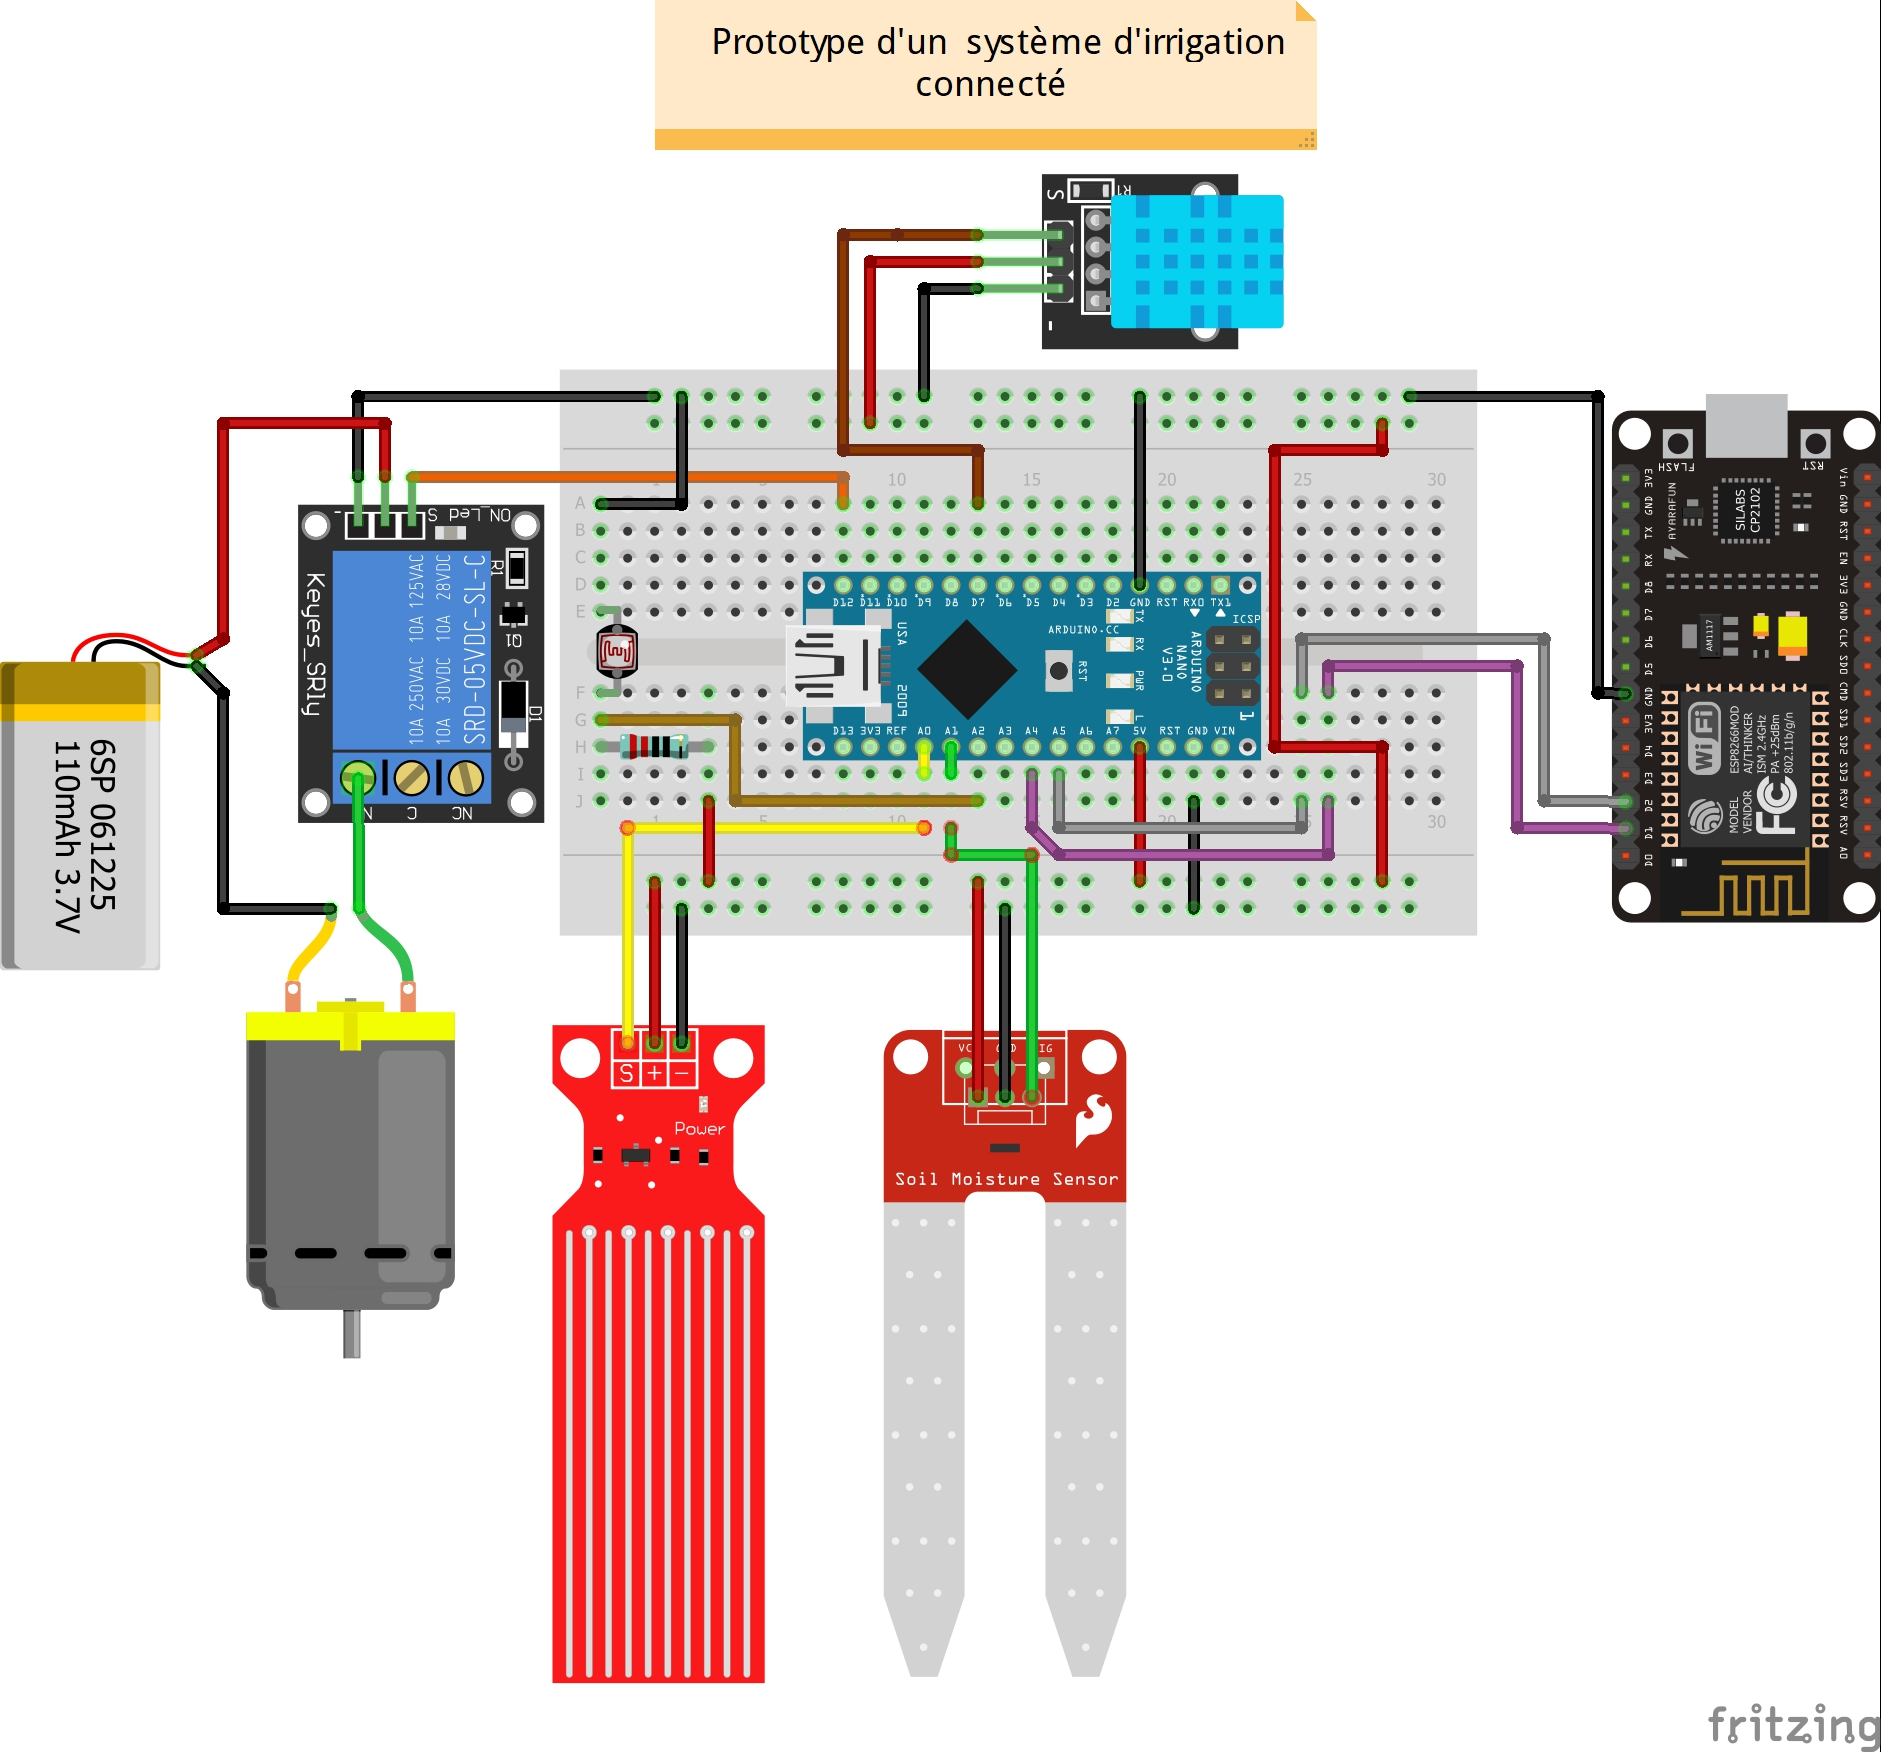
\includegraphics{chapitres/images/Irrigation_bb.jpg}
		\caption{Prototype du système d'irrigation connecté}
		\label{fig:labelname}
	\end{figure}
	\newpage
	\subsection{\textcolor{green}{Connection du système au Firebase :}}
			\begin{figure}[h]
				\centering
				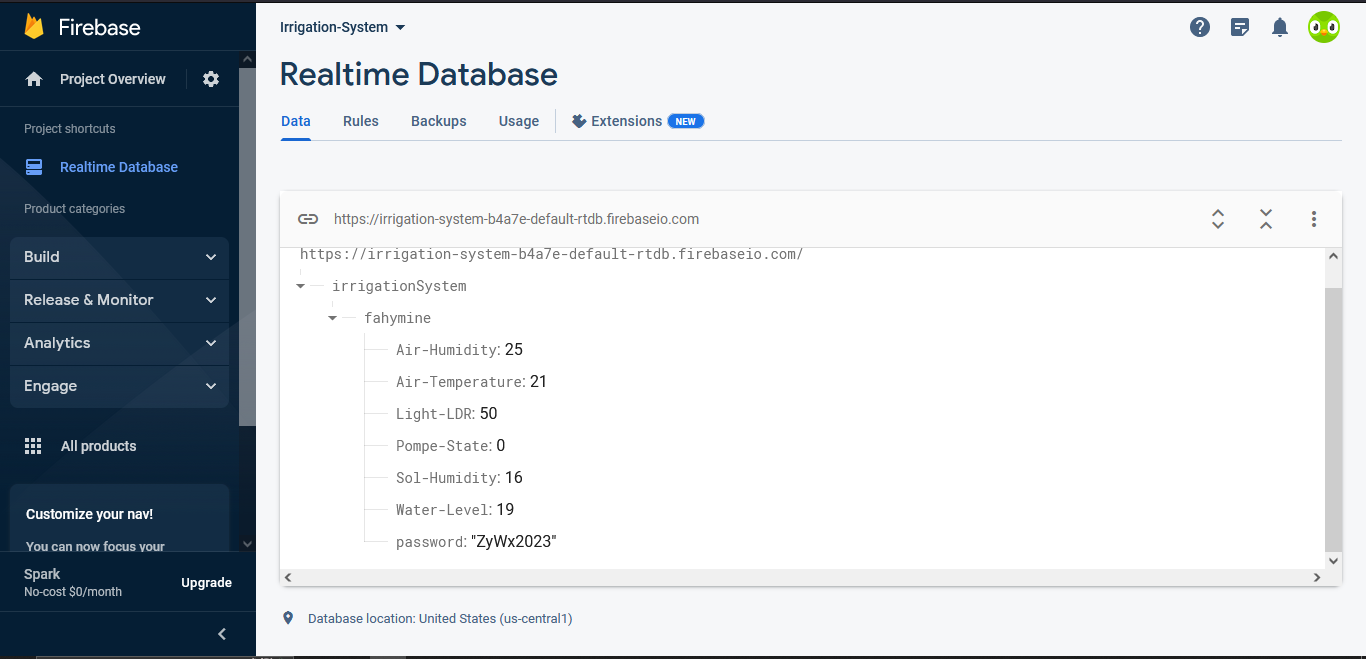
\includegraphics[width=0.9\textwidth]{chapitres/images/ConnectionEsp8266Firebase.PNG}
				\caption{Connection du système au Firebase}
				\label{fig:labelname}
			\end{figure}
	\newpage
	\subsection{\textcolor{green}{Programmation de la carte Arduino et de la NodeMCU :}}
		\subsubsection{\textcolor{blue}{Communication I2C code NodeMCU (dispositif maître) :}}
		\begin{lstlisting}[style=CStyle]
			#include <Wire.h>
			
			void setup() {
				Serial.begin(9600); /* begin serial for debug */
				Wire.begin(D1, D2); /* join i2c bus with SDA=D1 and SCL=D2 of NodeMCU */
			}
			
			void loop() {
				Wire.beginTransmission(8); /* begin with device address 8 */
				Wire.write("Hello Arduino");  /* sends hello string */
				Wire.endTransmission();    /* stop transmitting */
				
				Wire.requestFrom(8, 13); /* request & read data of size 13 from slave */
				while(Wire.available()){
					char c = Wire.read();
					Serial.print(c);
				}
				Serial.println();
				delay(1000);
			}
		\end{lstlisting}
	
	\subsubsection{\textcolor{blue}{Communication I2C code Arduino Uno (périphérique esclave) :}}
	\begin{lstlisting}[style=CStyle]
		#include <Wire.h>
		
		void setup() {
			Wire.begin(8);                /* join i2c bus with address 8 */
			Wire.onReceive(receiveEvent); /* register receive event */
			Wire.onRequest(requestEvent); /* register request event */
			Serial.begin(9600);           /* start serial for debug */
		}
		
		void loop() {
			delay(100);
		}
		
		// function that executes whenever data is received from master
		void receiveEvent(int howMany) {
			while (0 <Wire.available()) {
				char c = Wire.read();      /* receive byte as a character */
				Serial.print(c);           /* print the character */
			}
			Serial.println();             /* to newline */
		}
		
		// function that executes whenever data is requested from master
		void requestEvent() {
			Wire.write("Hello NodeMCU");  /*send string on request */
		}
	\end{lstlisting}
			
	

	\subsubsection{\textcolor{blue}{DHT11 et Arduino nano :}}
	\begin{lstlisting}[style=CStyle]
		// Read DHT11 sensor and send serially to PC
		
		#include <DHT.h>         // Include Adafruit DHT11 Sensors Library
		
		#define DHTPIN 7          // DHT11 Output Pin connection
		#define DHTTYPE DHT11     // DHT Type is DHT11
		
		DHT dht(DHTPIN, DHTTYPE);   // Initialize DHT sensor
		
		void setup () {
			dht.begin();
			Serial.begin(9600);         // To see data on serial monitor
		}
		
		void loop (){
			
			float H = dht.readHumidity();     //Read Humidity
			float T = dht.readTemperature();    // Read temperature as Celsius
			
			// Check if any reads failed and if exit
			if (isnan(H) || isnan(T)){
				Serial.println("Failed to read from DHT sensor!");
				return;
			}
			
			// Combine Humidity and Temperature into single string
			String dhtData = String(H) + "," + String(T);
			Serial.println(dhtData);
			delay(2000);   // Wait two seconds between measurements
		}
		
	\end{lstlisting}
	
	\subsubsection{\textcolor{blue}{Capteur d’humidité du sol Arduino nano  :}}
	\begin{lstlisting}[style=CStyle]
		#define solPin A1 // port de connexion du capteur
		
		int minsol = 300; 
		int sol;
		
		void setup(){
			Serial.begin(9600);
		}
		
		void loop(){
			sol = analogRead(solPin);
			Serial.print("sol = ");
			Serial.println(sol); // afficher variable	
			delay(1000);
		}
	\end{lstlisting}
	
	\subsubsection{\textcolor{blue}{Capteur de niveau d’eau Arduino  :}}
	\begin{lstlisting}[style=CStyle]
		int water;
		
		void setup() {
			pinMode(A0, INPUT);
			Serial.begin(9600); 
		}
		
		void loop() {
			water = analogRead(A0);
			Serial.println(water);
			
			delay(1000); // attend une seconde
		}
	\end{lstlisting}

		\subsubsection{\textcolor{blue}{LDR et Arduino nano :}}
	\begin{lstlisting}[style=CStyle]
		const int ldrPin = A2;
		int ldrValue = 0;
		
		void setup() {
			Serial.begin(9600);
		}
		
		void loop() {
			ldrValue = analogRead(ldrPin);
			Serial.println("ldrValue");
			Serial.println(ldrValue);
			delay(20);
		}
	\end{lstlisting}
		
	\subsection{\textcolor{green}{Réalisation finale du projet :}}
		\begin{figure}[h]
			\centering
			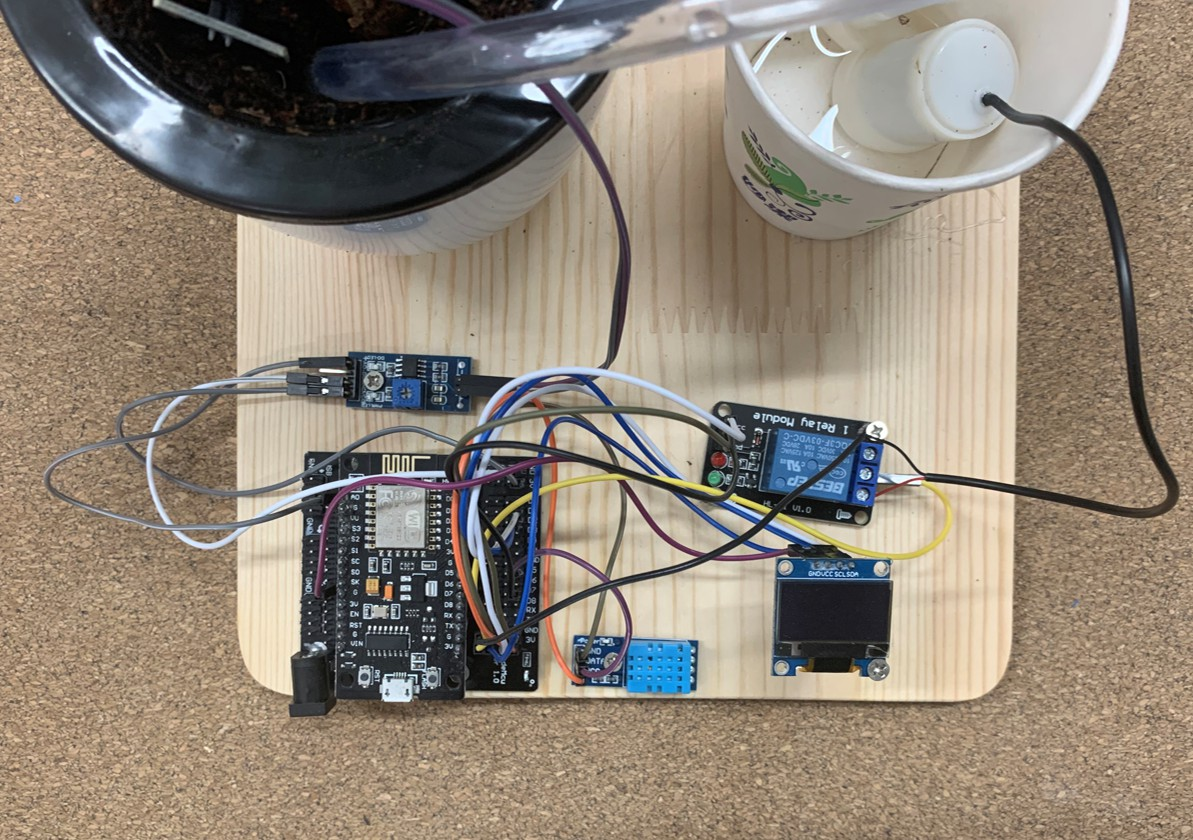
\includegraphics{chapitres/images/Realisation.jpg}
			\caption{Réalisation finale du projet}
			\label{fig:labelname}
		\end{figure}
	\newpage
	\subsection{\textcolor{green}{L’application Android Smart Agri:}}
	L’application mobile Smart Agri est développer en utilisant la framework flutter avec le langage de programmation Dart constitue de 5 fenêtres .
	\begin{itemize}
		\item \underline{Fenêtre 1} :
	\end{itemize}
	Cette fenêtre est faite en raison de sécurité de l’application pour qu’elle ne soit pas utilisée par n’importe qui. Il faut donc saisir un nom d’utilisateur et un mot  de passe correcte pour accéder aux autres fonctionnalités de l’application.
	\begin{figure}[h]
		\centering
		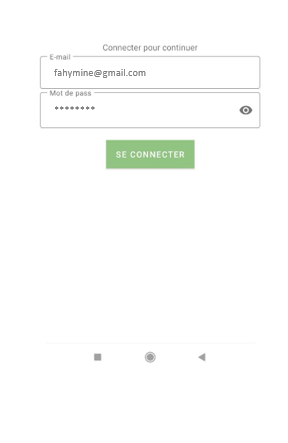
\includegraphics{chapitres/images/fenetre1.PNG}
		\caption{Interface d'accueil de l'application Smart Agri(Fenêtre 1)}
		\label{fig:labelname}
	\end{figure}
	\newpage
	\begin{itemize}
		\item \underline{Fenêtre 2} :
	\end{itemize} 
	Cette fenêtre est consacrée à afficher les différentes valeurs des capteurs et la commande de la  pompe. 
	Les dernières valeurs ajouter dans la base de données sont afficher ici.
	\newpage 
	\begin{figure}[h]
		\centering
		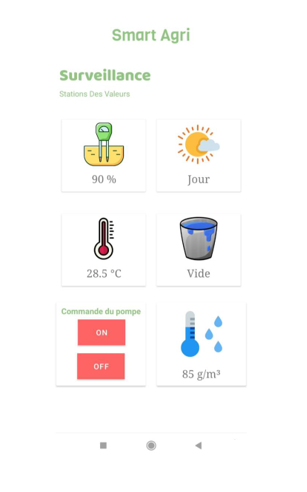
\includegraphics{chapitres/images/fenetre2.PNG}
		\caption{Interface d'affichage des données de l’application Smart Agri (Fenêtre 2)}
		\label{fig:labelname}
	\end{figure}
	\begin{itemize}
		\item \underline{Fenêtres 3, 4 et 5} :
	\end{itemize}
	Ces fenêtres sont consacrées à afficher la représentation graphique des valeurs de température, 
	humidité et humidité de sol. Seules les 20 dernières valeurs dans la base de données son afficher 
	dans ces fenêtres pour bien visualiser les données. Pour accéder au graphe souhaiter il suffit de 
	cliquer sur le carreau avec le symbole qui représente la donnée dans la fenêtre principale.
	\newpage
	\begin{figure}[h]
		\centering
		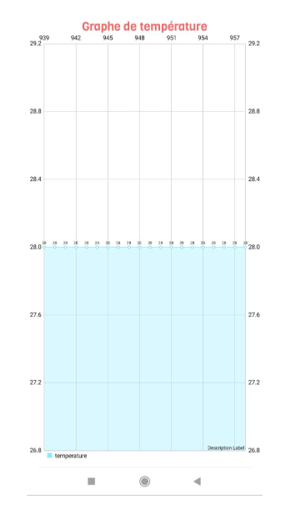
\includegraphics{chapitres/images/fenetre3.PNG}
		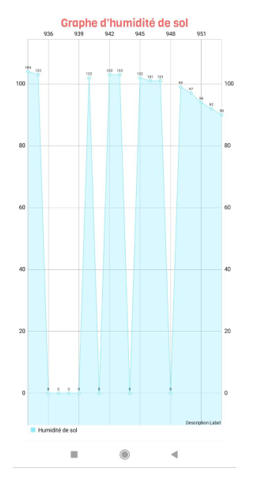
\includegraphics{chapitres/images/fenetre4.PNG}
		
	\end{figure}
	\begin{figure}[h]
		\centering
		
		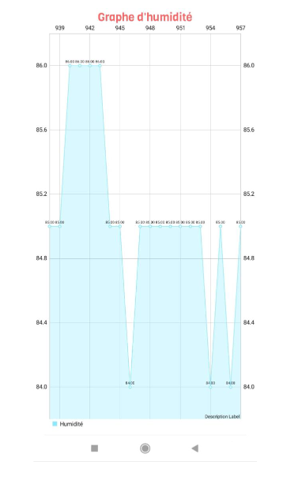
\includegraphics{chapitres/images/fenetre5.PNG}
		\caption{Interfaces de la représentation graphique du température, humidité de sol et humidité d'aire}
		\label{fig:labelname}
	\end{figure}
	
	\newpage
\end{flushleft}